\documentclass[tikz,border=6pt]{standalone}
\usetikzlibrary{arrows.meta,positioning,calc,fit}
\makeatletter
\AtBeginDocument{\global\let\pgf@selectfontorig\relax}
\makeatother

\tikzset{
  state/.style={
    draw=black,
    rounded corners=4pt,
    very thick,
    fill=white,
    minimum width=8.5mm,
    minimum height=7mm,
    align=center,
    inner sep=1.6pt,
    font=\scriptsize
  },
  initial/.style={-Latex, very thick},
  edge/.style={-Latex, thick, shorten >=2pt, shorten <=2pt},
  labelbox/.style={fill=white, inner sep=0.8pt, font=\tiny, scale=0.62, transform shape, align=center},
  panel/.style={draw=gray!70, rounded corners=6pt, very thick},
  title/.style={fill=white, inner sep=1.5pt, font=\itshape\large}
}

\newcommand{\initarrow}[2]{\draw[initial] #1 -- (#2);}

\newcommand{\panel}[3]{
  \node[panel, fit=#1, inner sep=6mm] (#2) {};
  \node[title, anchor=north west] at (#2.north west) {$#3$};
}

\begin{document}
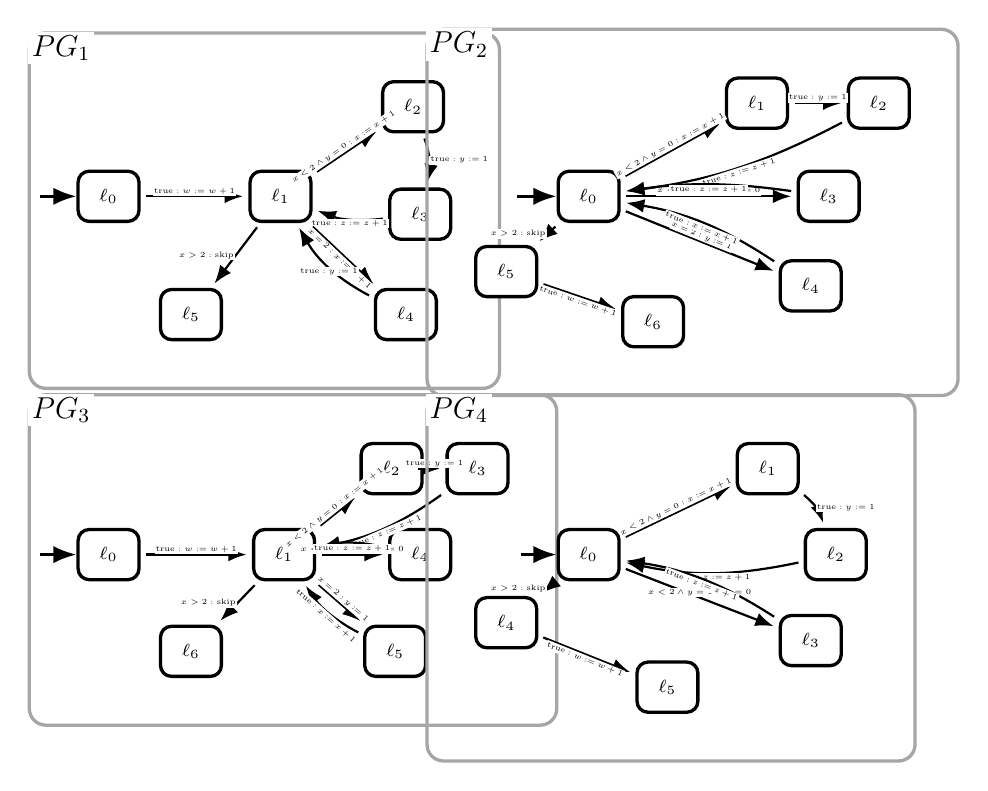
\begin{tikzpicture}[scale=0.91, transform shape]

  % -------------------------------------------------------------------
  % PG1
  % -------------------------------------------------------------------
  \begin{scope}[shift={(0,0)}]
    \node[state] (p10) at (0,0) {$\ell_0$};
    \node[state] (p11) at (2.4,0) {$\ell_1$};
    \node[state] (p12) at (4.25,1.25) {$\ell_2$};
    \node[state] (p13) at (4.35,-0.25) {$\ell_3$};
    \node[state] (p14) at (4.15,-1.65) {$\ell_4$};
    \node[state] (p15) at (1.15,-1.65) {$\ell_5$};
    \initarrow{(-0.95,0)}{p10.west}
    \draw[edge] (p10) -- node[labelbox, above] {$\mathrm{true}:w:=w+1$} (p11);
    \draw[edge] (p11) -- node[labelbox, above, sloped] {$x<2\land y=0:x:=x+1$} (p12);
    \draw[edge, bend left=16] (p12) to node[labelbox, right] {$\mathrm{true}:y:=1$} (p13);
    \draw[edge, bend left=14] (p13) to node[labelbox, below] {$\mathrm{true}:z:=z+1$} (p11);
    \draw[edge] (p11) -- node[labelbox, below, sloped] {$x=2:x:=x+1$} (p14);
    \draw[edge, bend left=16] (p14) to node[labelbox, below] {$\mathrm{true}:y:=1$} (p11);
    \draw[edge] (p11) -- node[labelbox, left] {$x>2:\mathrm{skip}$} (p15);
    \panel{(p10)(p11)(p12)(p13)(p14)(p15)}{pgonebox}{PG_1}
  \end{scope}

  % -------------------------------------------------------------------
  % PG2
  % -------------------------------------------------------------------
  \begin{scope}[shift={(6.7,0)}]
    \node[state] (p20) at (0,0) {$\ell_0$};
    \node[state] (p21) at (2.35,1.3) {$\ell_1$};
    \node[state] (p22) at (4.05,1.3) {$\ell_2$};
    \node[state] (p23) at (3.35,0) {$\ell_3$};
    \node[state] (p24) at (3.1,-1.25) {$\ell_4$};
    \node[state] (p25) at (-1.15,-1.05) {$\ell_5$};
    \node[state] (p26) at (0.9,-1.75) {$\ell_6$};
    \initarrow{(-1.0,0)}{p20.west}
    \draw[edge] (p20) -- node[labelbox, above, sloped] {$x<2\land y=0:x:=x+1$} (p21);
    \draw[edge] (p21) -- node[labelbox, above] {$\mathrm{true}:y:=1$} (p22);
    \draw[edge, bend left=10] (p22) to node[labelbox, below, sloped] {$\mathrm{true}:z:=z+1$} (p20);
    \draw[edge] (p20) -- node[labelbox, above] {$x<2\land y=1:y:=0$} (p23);
    \draw[edge, bend right=8] (p23) to node[labelbox, below] {$\mathrm{true}:z:=z+1$} (p20);
    \draw[edge] (p20) -- node[labelbox, above, sloped] {$x=2:y:=1$} (p24);
    \draw[edge, bend right=12] (p24) to node[labelbox, below, sloped] {$\mathrm{true}:x:=x+1$} (p20);
    \draw[edge] (p20) -- node[labelbox, left] {$x>2:\mathrm{skip}$} (p25);
    \draw[edge] (p25) -- node[labelbox, below, sloped] {$\mathrm{true}:w:=w+1$} (p26);
    \panel{(p20)(p21)(p22)(p23)(p24)(p25)(p26)}{pgtwobox}{PG_2}
  \end{scope}

  % -------------------------------------------------------------------
  % PG3
  % -------------------------------------------------------------------
  \begin{scope}[shift={(0,-5.0)}]
    \node[state] (p30) at (0,0) {$\ell_0$};
    \node[state] (p31) at (2.45,0) {$\ell_1$};
    \node[state] (p32) at (3.95,1.2) {$\ell_2$};
    \node[state] (p33) at (5.15,1.2) {$\ell_3$};
    \node[state] (p34) at (4.35,0) {$\ell_4$};
    \node[state] (p35) at (4.0,-1.35) {$\ell_5$};
    \node[state] (p36) at (1.15,-1.35) {$\ell_6$};
    \initarrow{(-0.95,0)}{p30.west}
    \draw[edge] (p30) -- node[labelbox, above] {$\mathrm{true}:w:=w+1$} (p31);
    \draw[edge] (p31) -- node[labelbox, above, sloped] {$x<2\land y=0:x:=x+1$} (p32);
    \draw[edge] (p32) -- node[labelbox, above] {$\mathrm{true}:y:=1$} (p33);
    \draw[edge, bend left=12] (p33) to node[labelbox, below, sloped] {$\mathrm{true}:z:=z+1$} (p31);
    \draw[edge] (p31) -- node[labelbox, above] {$x<2\land y=1:y:=0$} (p34);
    \draw[edge, bend right=12] (p34) to node[labelbox, below] {$\mathrm{true}:z:=z+1$} (p31);
    \draw[edge] (p31) -- node[labelbox, above, sloped] {$x=2:y:=1$} (p35);
    \draw[edge, bend left=14] (p35) to node[labelbox, below, sloped] {$\mathrm{true}:x:=x+1$} (p31);
    \draw[edge] (p31) -- node[labelbox, left] {$x>2:\mathrm{skip}$} (p36);
    \panel{(p30)(p31)(p32)(p33)(p34)(p35)(p36)}{pgthreebox}{PG_3}
  \end{scope}

  % -------------------------------------------------------------------
  % PG4
  % -------------------------------------------------------------------
  \begin{scope}[shift={(6.7,-5.0)}]
    \node[state] (p40) at (0,0) {$\ell_0$};
    \node[state] (p41) at (2.5,1.2) {$\ell_1$};
    \node[state] (p42) at (3.45,0) {$\ell_2$};
    \node[state] (p43) at (3.1,-1.2) {$\ell_3$};
    \node[state] (p44) at (-1.15,-0.95) {$\ell_4$};
    \node[state] (p45) at (1.1,-1.85) {$\ell_5$};
    \initarrow{(-0.95,0)}{p40.west}
    \draw[edge] (p40) -- node[labelbox, above, sloped] {$x<2\land y=0:x:=x+1$} (p41);
    \draw[edge, bend left=16] (p41) to node[labelbox, right] {$\mathrm{true}:y:=1$} (p42);
    \draw[edge, bend left=12] (p42) to node[labelbox, below] {$\mathrm{true}:z:=z+1$} (p40);
    \draw[edge] (p40) -- node[labelbox, above] {$x<2\land y=1:y:=0$} (p43);
    \draw[edge, bend right=12] (p43) to node[labelbox, below, sloped] {$\mathrm{true}:z:=z+1$} (p40);
    \draw[edge] (p40) -- node[labelbox, left] {$x>2:\mathrm{skip}$} (p44);
    \draw[edge] (p44) -- node[labelbox, below, sloped] {$\mathrm{true}:w:=w+1$} (p45);
    \panel{(p40)(p41)(p42)(p43)(p44)(p45)}{pgfourbox}{PG_4}
  \end{scope}

\end{tikzpicture}
\end{document}
